\documentclass[a4paper]{article}
\usepackage[utf8]{inputenc}
\usepackage[russian,english]{babel}
\usepackage[T2A]{fontenc}
\usepackage[left=10mm, top=20mm, right=18mm, bottom=15mm, footskip=10mm]{geometry}
\usepackage{indentfirst}
\usepackage{amsmath,amssymb}
\usepackage[italicdiff]{physics}
\usepackage{graphicx}
\graphicspath{{images/}}
\DeclareGraphicsExtensions{.pdf,.png,.jpg}
\usepackage{wrapfig}

\usepackage{caption}
\captionsetup[figure]{name=Рисунок}
\captionsetup[table]{name=Таблица}
  
\title{\underline{Отчет о выполненой лабораторной работе 1.3.1}}
\author{Антон Хмельницкий, Б01-306}


\begin{document}

\maketitle
\textbf{Определение модуля Юнга на основе исследования деформаций растяжения и изгиба}

\section{Аннотация}
    \par \textbf{Цель работы:} экспериментально получить зависимость между напряжением и деформацией
    для двух простейших напряженных состояний упругих тел: одностороннего сжатия и чистого изгиба;
    по результатам эксперимента вычислить модул Юнга.\\
    \par \noindent \textbf{В работе используются:} в первой части - прибор Лермантова, проволока
    из исследуемого материала,
     зрительная трубка со шкалой,
    набор грузов, микрометр, рулетка;  во второй части - стойка для изгибания балки, индикатор для
    измерения величин прогиба,
набор исследуемых стержней, грузы, линейка, штангенциркуль.


\section{Определение модуля Юнга по измерению изгиба балки}

\subsection{Теоретические сведения}
Модуль Юнга материала стержня $E$ связан со стрелой прогиба $y_{max}$ как:
\begin{equation}\label{balka}
    E=\frac{Pl^3}{4ab^3y_{max}}
\end{equation}
где $P$ - нагрузка на стержень, $l$ - расстояние меду точками опоры,
$a$ - ширина балки ,$b$ - высота балки

\subsection{Экспериментальная установка}

\begin{figure}[!ht]
    \centering
    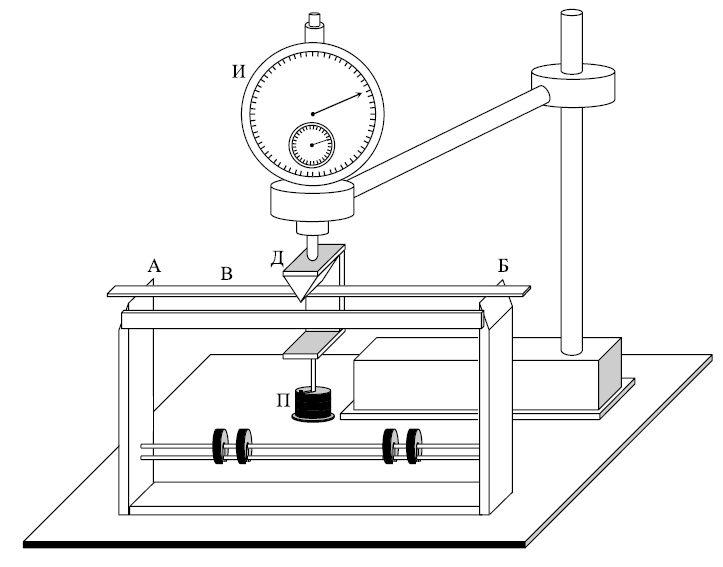
\includegraphics[scale=0.8]{balka.png}
    \caption{Установка для измерения модуля Юнга}
\end{figure}

Экспериментальная установка состоит из прочной стойки с опорными призмами А и Б (рис. 2). На ребра призм опирается исследуемый
стержень (балка) В. В середине стержня на призме Д подвешена площадка П с грузами. Измерять стрелу прогиба можно с помощью индикатора И, укрепляемого на отдельной штанге. Полный оборот большой стрелки индикатора соответствует 1 мм и одному делению малого циферблата.

\newpage
\subsection{Расчет всех данных}

В данной уставновке $l = 50,2$ см

\begin{table}[h!]
\begin{center}
\begin{tabular}{|c|c|}
\hline
Ширина, $a$, см & Толщина, $b$, см \\ \hline
1,98       & 1,1         \\ \hline
1,99       & 1,075       \\ \hline
2          & 1,05        \\ \hline
1,99       & 1,07        \\ \hline
2          & 1,03        \\ \hline
2          & 1,06        \\ \hline
1,8        & 1,085       \\ \hline
1,6        & 1,73        \\ \hline
2          & 1,078       \\ \hline
1,99       & 1,065       \\ \hline
\end{tabular}
\caption{Измерение средней ширины и толцины балки}
\end{center}
\end{table}

Для измеренных значений среднее будет $\overline{a} = 1,934 $ см и $\overline{b} = 1,064$ см.
Для $a$:
\begin{itemize}
\item Среднее значение: $\langle a \rangle = \frac{1}{n}\sum\limits_{i=1}^n a_{i} = 1,934$ см. 
\item Стандартное отклонение: $\sigma_{a} = \sqrt{\frac{1}{n}\sum\limits_{i=1}^n(a_{i} - \langle a \rangle)^2} = 0.126$ см.
\item Стандартная погрешность опыта: $\sigma_\text{ср} = \frac{\sigma_{\text{a}}}{\sqrt{n}} =  0,04$ см.
\item Полная погрешность: $\sigma_{\text{полн}} = \sqrt{\sigma_{\text{случ}}^2 + \sigma_{a}^2} = 0.041$ мм.
\end{itemize}
Для $b$:
\begin{itemize}
\item Среднее значение: $\langle b \rangle = \frac{1}{n}\sum\limits_{i=1}^n b_{i} = 1,064$ см. 
\item Стандартное отклонение: $\sigma_{b} = \sqrt{\frac{1}{n}\sum\limits_{i=1}^n(b_{i} - \langle b \rangle)^2} = 0.021$ см.
\item Стандартная погрешность опыта: $\sigma_\text{ср} = \frac{\sigma_{b}}{\sqrt{n}} =  0,007$ см.
\item Полная погрешность: $\sigma_{\text{полн}} = \sqrt{\sigma_{\text{случ}}^2 + \sigma_{b}^2} = 0,012$ мм.
\end{itemize}
Итоговые результаты: \par
$a = 1,934 \pm 0,041 (\varepsilon_{a} = 2,1\%)$\\
$b = 1,064 \pm 0,012 (\varepsilon_{b} = 1,1\%)$

При измерении балка не возвращалась на прежнее положение

\begin{table}[h!]
\begin{center}
\begin{tabular}{|cc|}
\hline
\multicolumn{2}{|c|}{Если сместить центр на 5мм} \\ \hline
\multicolumn{1}{|c|}{$M$, гр}   & $y_{max}$, мм  \\ \hline
\multicolumn{1}{|c|}{503,1}     & 0,56           \\ \hline
\multicolumn{1}{|c|}{467,9}     & 0,53           \\ \hline
\multicolumn{1}{|c|}{482,5}     & 0,54           \\ \hline
\end{tabular}
\end{center}
\end{table}

\begin{table}[h!]
\begin{center}
\begin{tabular}{|c|c|c|}
\hline
$M$, гр & $P$, Н   & $y_{max}$, мм \\ \hline
511     & 5,0078   & 0,629         \\ \hline
482,5   & 4,7285   & 0,6           \\ \hline
503,3   & 4,93234  & 0,61          \\ \hline
467,9   & 4,58542  & 0,595         \\ \hline
503,1   & 4,93038  & 0,62          \\ \hline
971     & 9,5158   & 1,2           \\ \hline
1014,3  & 9,94014  & 1,231         \\ \hline
985,6   & 9,65888  & 1,235         \\ \hline
1004,4  & 9,84312  & 1,205         \\ \hline
1494,8  & 14,64904 & 1,815         \\ \hline
\end{tabular}
\caption{Данные для зависимости $P(y_{max})$ для деревянной балки с одной стороны}
\end{center}
\end{table}

\begin{table}[h!]
\begin{center}
\begin{tabular}{|c|c|c|}
\hline
$M$, гр & $P$, Н  & $y_{max}$, мм \\ \hline
467,9   & 4,58542 & 0,719         \\ \hline
503,1   & 4,93038 & 0,827         \\ \hline
511     & 5,0078  & 0,871         \\ \hline
466,7   & 4,57366 & 0,787         \\ \hline
503,3   & 4,93234 & 0,9           \\ \hline
482,5   & 4,7285  & 0,81          \\ \hline
501,3   & 4,91274 & 0,93          \\ \hline
478,2   & 4,68636 & 0,86          \\ \hline
461,8   & 4,52564 & 0,87          \\ \hline
\end{tabular}
\caption{Данные для зависимости $P(y_{max})$ для деревянной балки с другой стороны}
\end{center}
\end{table}

\newpage
\subsection{Обработка результатов}

Расчет погрешность при аппроксимации по МНК:

\[k=\frac{\langle xy\rangle-\langle x\rangle \langle y\rangle}{\langle x^2\rangle - \langle x\rangle^2}\]
\[\sigma_{k} = \frac{1}{\sqrt{N}}\sqrt{\frac{\langle y^2 \rangle - \langle y \rangle ^2}{\langle x^2 \rangle - \langle x \rangle ^2} - k^2}\]\\
Тогда для одной стороны $k_{1} = 8.074 \pm 0,0736 (\varepsilon_{k_{1}} \approx 0,91\%)$.\\
Для другой стороны $k_{2} = 5,467 \pm 0,32 (\varepsilon_{k_{2}} \approx 6\%)$.

Модуль Юнга:
\begin{equation}
    E = \frac{Pl^3}{4\overline{a}(\overline{b})^3 y_{max}} = k\frac{l^3}{4\overline{a}(\overline{b})^3}
\end{equation}
Погрешность:
\[
    \varepsilon_{E} = \sqrt{(\varepsilon_{k})^2 + (3\varepsilon_{l})^2 + (\varepsilon_{a})^2 + (3\varepsilon_{b})^2}
\]
\begin{table}[h!]
\begin{center}
\begin{tabular}{|c|c|c|c|c|c|}
\hline
$\sigma_{a}$ & 0,1 мм & $a$ & 1,934 см   & $\varepsilon_{a}$ & $2,1\%$  \\ \hline
$\sigma_{b}$ & 0,1 мм & $b$ & 1,06 см    & $\varepsilon_{b}$ & $1,1\%$ \\ \hline
$\sigma_{l}$ & 1 мм   & $l$ & 50,2 см    & $\varepsilon_{l}$ & $0,2\%$  \\ \hline
$\sigma_{k}$ & 0,074  & $k$ & 8,074 Н/мм & $\varepsilon_{k}$ & $0,92\%$ \\ \hline
\end{tabular}
\caption{Погрешности}
\end{center}
\end{table}
Получаем $\varepsilon_{E} = 4,1\%$ и $E = 10,96$ ГПа. 

\begin{figure}[p]
    \centering
    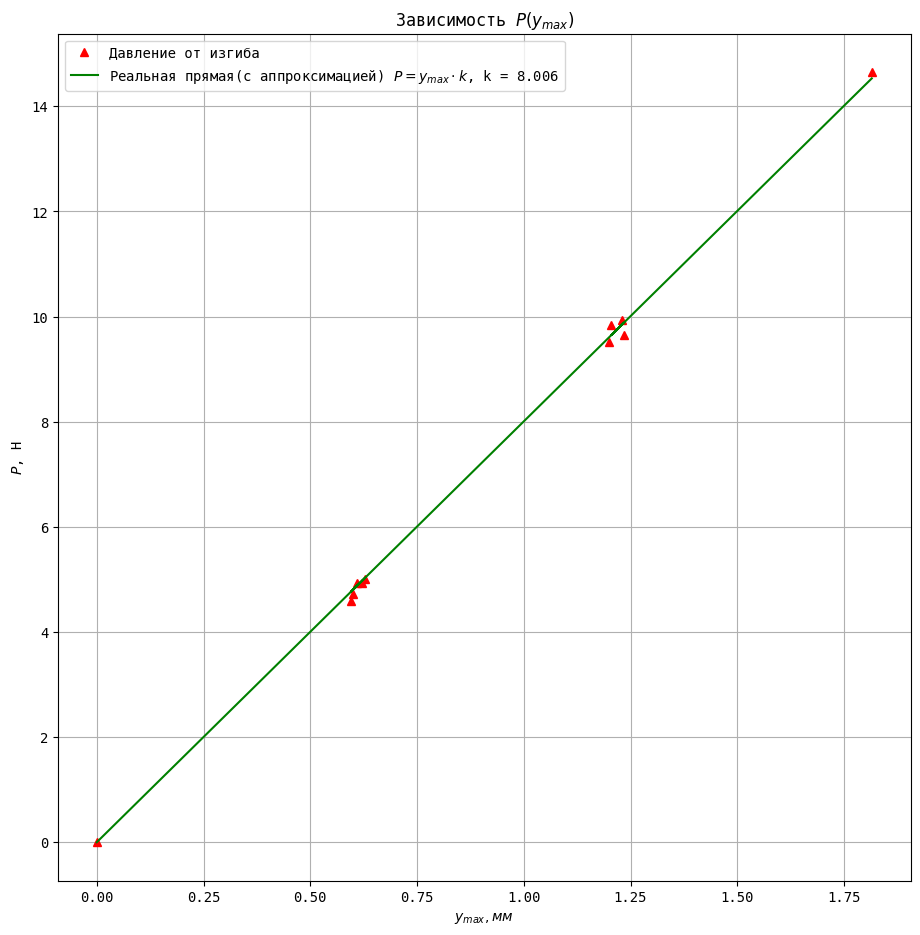
\includegraphics[scale=0.8]{graphic1.png}
    \caption{График для деревянной балки с одной стороны}
\end{figure}

\begin{figure}[p]
    \centering
    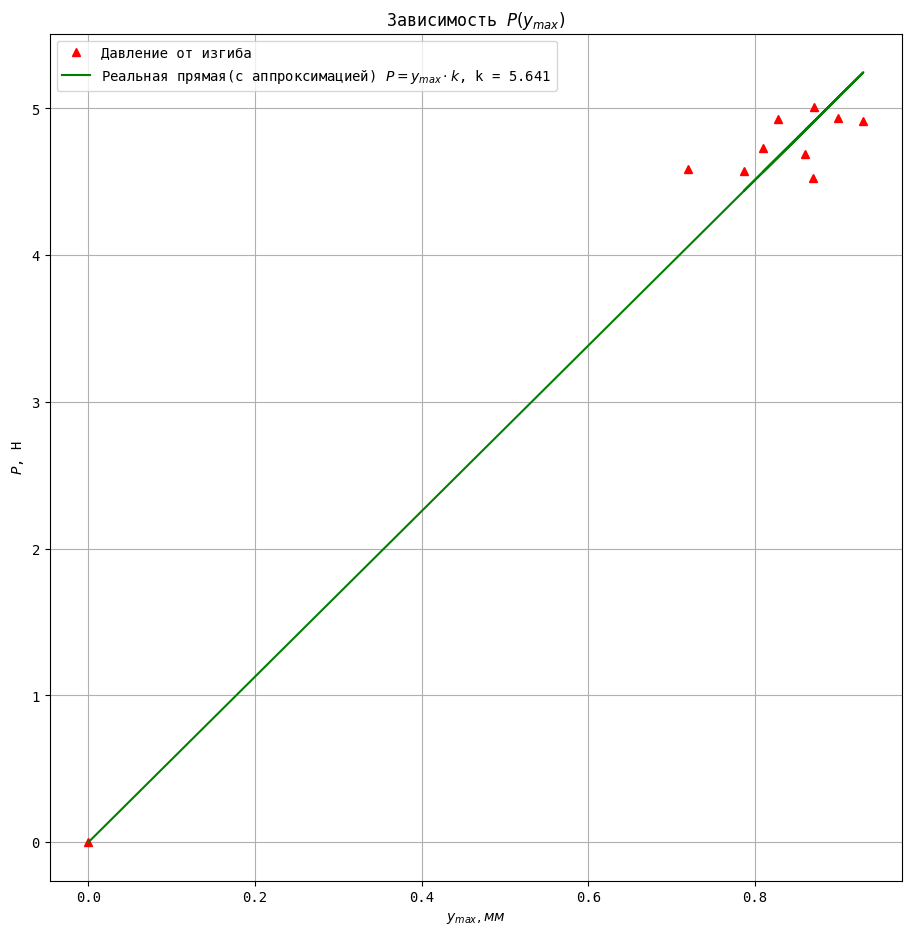
\includegraphics[scale=0.8]{graphic2.png}
    \caption{График для деревянной балки с другой стороны}
\end{figure}


\newpage
\section{Выводы}

В работе была исследована зависимость между напряжением и деформацией балки и измерен модуль Юнга для дерева.\\
Сравнивая полученное значение $E = 10,96 \pm 0,45 \text{ ГПа } (\varepsilon_{E} = 4,1\%)$ с табличным($E = 10,2$ ГПа) получаем, что оно лежит в пределах $2\sigma_{E}$.

\end{document}
